\documentclass{hbrs-ecta-report}

\usepackage{float}
\usepackage{placeins}
\usepackage[utf8]{inputenc}
\usepackage{fontenc}
\usepackage{ngerman}

\begin{document}

\conferenceinfo{H-BRS}{2017}

\title{NeuroEvolution of Augmenting Topologies (NEAT)}
\subtitle{Steuerung eins Mario Jump \& Run Spiels}

\numberofauthors{2}
\author{
Jan Urfei\\
       \affaddr{Bonn-Rhein-Sieg University of Applied Sciences}\\
       \affaddr{Grantham-Allee 20}\\
       \affaddr{53757 Sankt Augustin, Germany}\\
       \email{jan.urfei@inf.h-brs.de}\\
\and
	Tim Lügger\\
	\affaddr{Bonn-Rhein-Sieg University of Applied Sciences}\\
	\affaddr{Grantham-Allee 20}\\
	\affaddr{53757 Sankt Augustin, Germany}\\
	\email{tim.luegger@inf.h-brs.de}\\
}
\date{today}
\maketitle
\begin{abstract}
Ziel war es eine Mario Spielfigur mit bestimmten Szenarien zu trainieren, sodass diese dann das/die Level best möglichst lösen kann.
\end{abstract}

%% ------------------------------ GENERAL NOTES ------------------------------ %%
\section{General Notes}
\label{sec:generalnotes}
\begin{itemize}
\item Do not state things you cannot confirm either by literature or experiment. This is science, not black magic.
\item Normalize your data and resulting statistical descriptors (like RMSE, $\mu$)
\item Save your experimental results to disk \textbf{before you visualize}. You \textbf{will} change your plots quite a lot after gathering the data.
\item Don't submit reports with many pages containing just a single figure. Scrolling is terrible for our health.
\item \textbf{Separate} training and test data. Don't use test data in your algorithm to learn or make decisions, they are only allowed to test the end result. If you need a separate sample set to make decisions during training or optimization, create a third (validation) set. Only your test data will really tell you how good your algorithm is. 
\end{itemize}

\subsection{Algorithm Parametrization}
Develop an actual strategy, preferably on a reduced but similar problem. You can reduce the number of samples, the targetted number of time steps your controller runs in a simulation, or any other non-destructive problem reduction method. If your algorithm has two paramers you need to adjust, it should be no problem to take 5 \textit{sensible} values per parameter and compare all combinations. For stochastic algorithms, like evolutionary approaches, make sure you \textbf{repeat your experiments} at least 5-10 times, depending on the amount of randomness. Since your algorithm makes "random" changes, just comparing single runs does not give you a good estimation on its performance. Do \textbf{not} pick your values such that they only confirm the values you \textbf{want} to use.

%% ------------------------------ STRUCTURE ------------------------------ %%
\subsection{Structure}
\label{sec:structure}
\begin{enumerate}
\item \textbf{Assignment Description}: first provide a brief description of the assignment that was handed out to you. This includes a description of the data.
\item \textbf{Approach}: describe the algorithm
\item \textbf{Experiments}: describe your experimental setup, algorithm parameters, data preprocessing first. Then include the results and a discussion thereof.
\item \textbf{Conclusion}: any conclusions about the algorithm, bugs, future work.
\end{enumerate}
%% ------------------------------ VISUALIZATION ------------------------------ %%
\subsection{Visualization}
\label{sec:visualization}

\begin{itemize}
\item Label your axes
\item Use logarithmic scale when appropriate
\item Use descriptive captions below your figures
\item Add legends if necessary
\item Make fontsizes large enough, linewidths thick enough to be readible in the final report.
\item When making comparisons, make sure the results are either in the \textbf{same} graph or graphs are plotted next to (or close to) each other.
\item \textbf{In short: make sure people can read your figures}
\end{itemize}

%% ------------------------------ REPORT STRUCTURE ------------------------------ %%
\FloatBarrier
\newpage
\newpage
\section{Assignment}
Aufgabe war es den für die HeartRate Prediction implementierten NEAT Algorithmus\cite{Stanley2002a} anzupassen, dass er ein Problem eines ausgesuchten Projektes löst.

In diesem Projekt wurde ein Simulator verwendet, der dem Jump\&Run Spiel Super Mario Bros. nachempfunden ist.
%todo cite simulator lib
Ziel diese Spieles ist eine Figur in einer 2D-Welt zu steuern und möglichst das Ende des Levels zu erreichen. Dabei existieren Hindernisse wie Schluchten oder Monster die es zu überwinden gilt. 

Zielsetzung war es zu ergründen, ob es NEAT erlaubt ein Netzwerk zu trainieren, welches basierend auf den Informationen aus dem aktuellen Sichtfeld die Spielfigur steuert, um ans Ende des (statischen) Levels zu gelangen.

Als Trainingsdaten wurde sich zunächst auf ein generiertes Level beschränkt, welches nur Blöcke, Schluchten oder erhöhte Ebenen enthielt, die es zu überspringen galt.

Das Sichtfeld beseht aus einem Gitter, zentriert um die Spielfigur herum (siehe Figure \ref{fig:MarioInput}). Die Objekte/Kacheln im Level unterscheiden sich anhand ihrem Typ (z.B Boden, Wand) und ihrer Position.

\begin{figure}[h!]
	\centering
	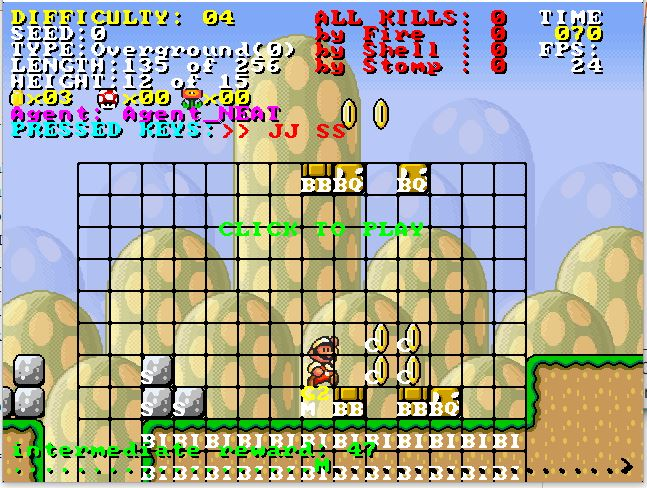
\includegraphics[width=\linewidth]{img/MarioInput.jpg}
	\caption{Umgebungsblöcke der Spielfigur für den Input}
	\label{fig:MarioInput} 
\end{figure}

\FloatBarrier
\section{Approach}
Im Gegensatz zum NEAT Paper \cite{Stanley2002a} wird eine Mutation verwendet, die Kanten wieder deaktivieren kann, damit die Topologien minimiert werden, falls nicht alle Eingaben aus dem Sichtfeld benötigt werden. 
Des weiteren wurde auf Fitnesssharing verzichtet.


Um die Kommunikation zwischen dem Simulator und Matlab herzustellen wurde die MATLAB API for Java verwendet. Diese erlaubt es aus Java heraus mit der Matlab Seesion zu interagieren.
In jeder Iteration wird die aktuelle Population aus dem Workspace geladen und bei der Ausführung des Simulators anhand des aktuellen Sichtfelds der Spielfigur der Output bzw. den daraus resultierenden Tastendruck. 
Um die Kommunikation zwischen Matlab und Java möglichst gering zu halten ist die Berechnung der Netze in Java mittels der Matrizen Bibliothek NDJ4 %todo cite
implementiert. 
Hat der die Spielfigur das Ende des Levels erreicht, ist die Spielzeit abgelaufen, die Spielfigur in eine Schlucht gefallen oder stecken/stehen geblieben wird die fitness auf den erreichten Levelfortschirtt gesetzt (x-Position). Außerdem wird bei Topologien, die das Ende des Levels erreichen, die restliche Spielzeit addiert um die Geschwindigkeit in der das Level abgeschlossen wird zu belohnen. Die Fitnesswerte werden zurück in den Matlab Workspace geschrieben und die Mutation mittels NEAT durchzuführen. Danach beginnt der Prozess von neuem. 
In der folgenden Abbildung (Figure \ref{fig:sequenzdiagramm}) ist der Ablauf nochmals veranschaulicht.

\begin{figure}[h!]
	\centering
	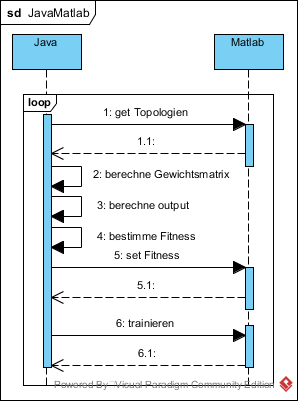
\includegraphics[width=\linewidth]{img/JavaMatlab.png}
	\caption{Kommunikation und Ablauf zwischen Java und Matlab}
	\label{fig:sequenzdiagramm} 
\end{figure}

Das Sichtfeld der Spielfigur ist auf 15x15 (Breite x Höhe) Felder begrenzt bzw. auf 7x15 also nur die rechte Hälfte des Sichtfeldes, da im ausgewählten Level keine Rückwertsbewegung notwendig ist.

Um die Eingabemenge gering zu halten wurden ähnliche Kacheln mit dem selben Eingabewert versehen (z.b Boden, Fels) sowie unwichtigeren Kacheln geringere Eingabegrößen vergeben.

\FloatBarrier
\section{Experiments}
Unsere Experimente sind jeweils 5 mal durchgeführt worden. Dabei wurden pro Experiment 1-2 Parameter verändert und getestet. Uns ist bewusst, dass 5 Wiederholungen eigentlich zu wenig sind, aber ein Experiment mit 5 Wiederholungen und jeweils 6 verschiedenen Parametrisierungen hat schon ca. 9h benötigt, was bei noch mehr Wiederholungen den Rahmen gesprengt hätte.

\subsection{Lernraten}
Mit dem Folgenden Experiment wurde ausgewertet, welche Einfluss die Lernrate bzw. die Wahl der Standardabweichung bei der Normalverteilung der Gewichtsmutation hat. Sowie die Auswirkungen des zufällige Zurücksetzen von Gewichten. 
Beispielsweise werden bei einer Gewichtsmutationsrate (wm) von 0.9, 90\% der zu mutierenden Gewichte mit einer normalverteilten Zufallszahl mit der angegebenen Standardabweichung (std) addiert. Die anderen 10\% werden zufällig neu gesetzt.

\begin{figure}[ht!]
	\centering
	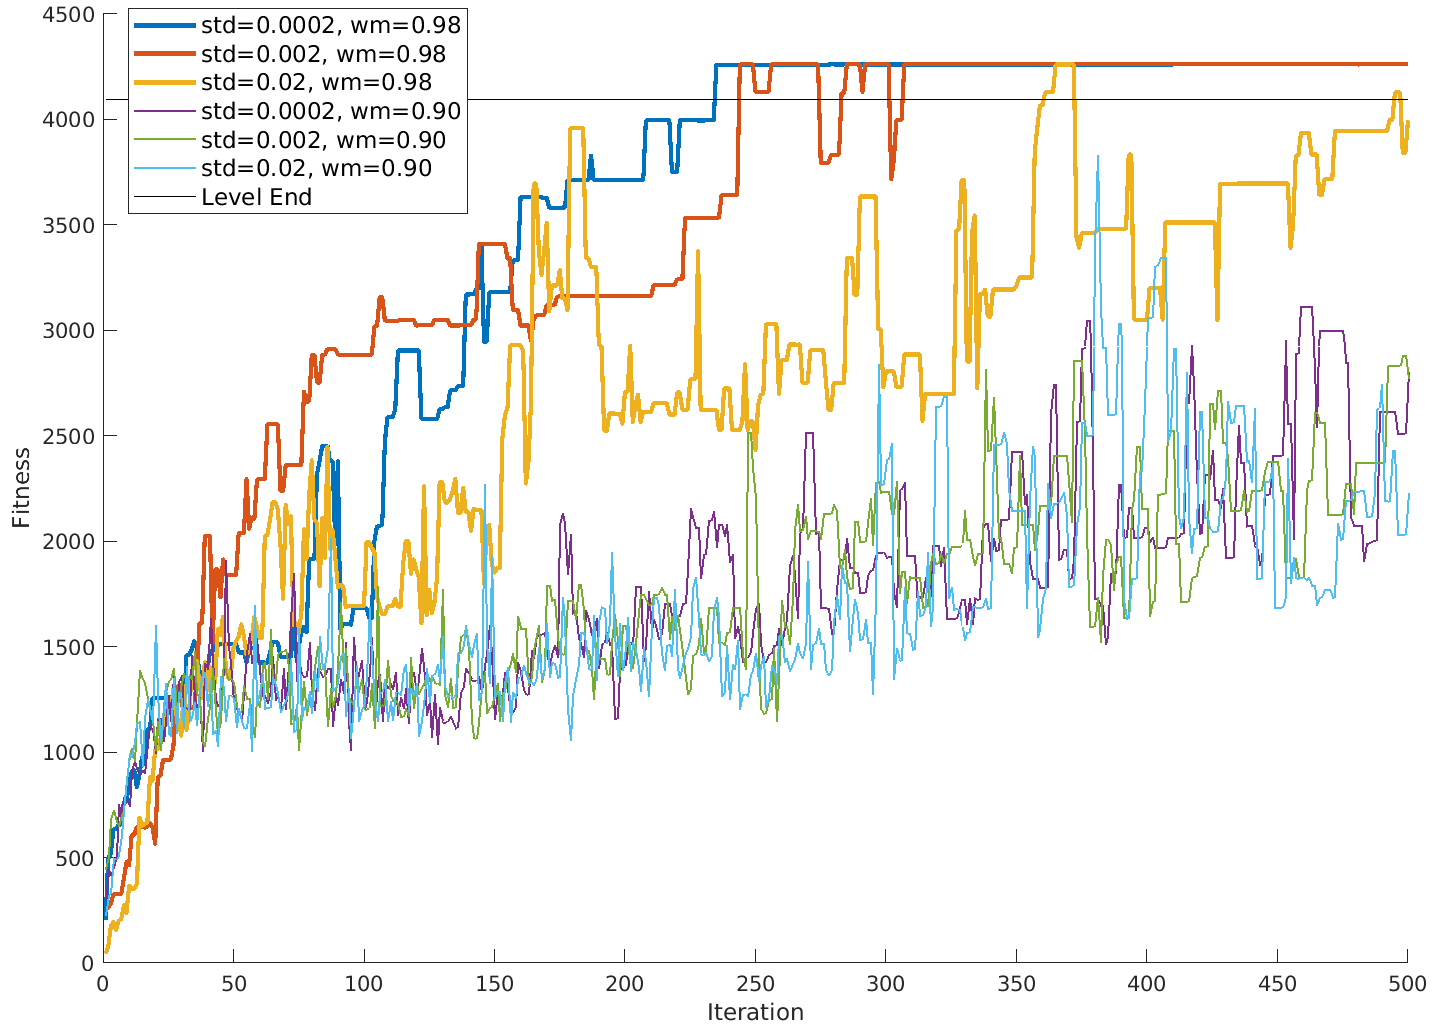
\includegraphics[width=\linewidth]{img/learningRates.png}
	\caption{Durchschnitt Elite Fitness}
	\label{fig:learningRates} 
\end{figure}

Man erkennt, dass wenn weniger Gewichte neu gewählt wurden, wesentlich früher Netze gefunden werden, welches das Level erfolgreich beenden.
Die Überschneidung der beiden Durchläufe std=0.0002, std=0.002 mit wm=0.98 deuten daraufhin, dass es sinnvoll gewesen wäre mit einer nicht zu geringen Standardabweichung zu starten diese dann aber ab ca. 100 Iterationen zu reduzieren.

\begin{figure}[h!]
	\centering
	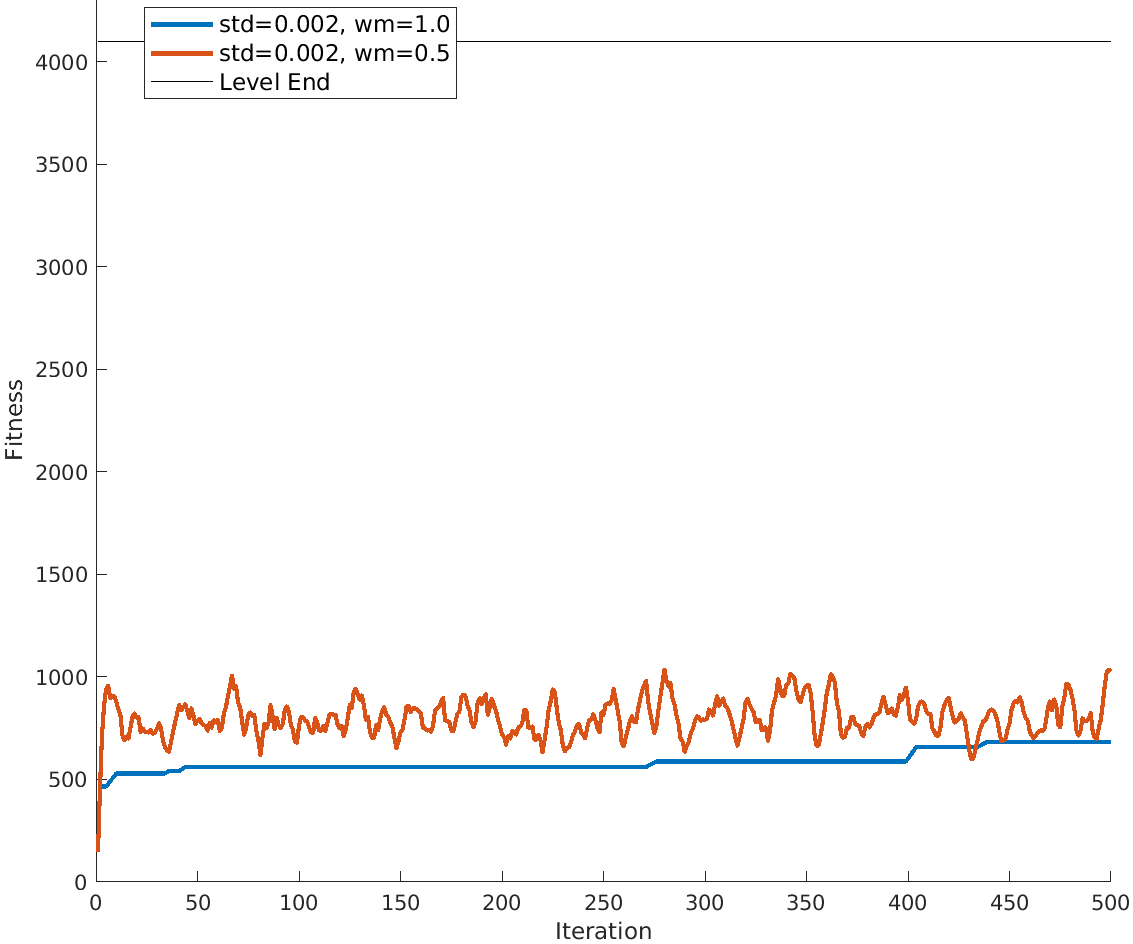
\includegraphics[width=\linewidth]{img/learningRates2.png}
	\caption{(Keine) Neuwahl der Gewichte}
	\label{fig:learningRates2} 
\end{figure}

Das zufällige neu Wählen der Gewichte ist essenziell für den Lernerfolg. Die Spielfigur schafft ansonsten im Level nur knapp über 500 Pixel weit. Werden zu viele Gewichte neu gewählt, variieren die Topologien zu stark, sodass sich kein großer Lerneffekt einstellt.

\subsection{Controls}
Im folgenden wurden verschiedene Varianten der Steuerung (Tastatureingaben) verglichen.
Mit der Predefined Methode wurde den Ausgabeneuronen Tastenkombinationen zugeordnet. In jedem Zeitschritt wird dann die, mit der aktuell höchsten Aktivierung, ausgeführt.
Bei der Threshold Methode wird jedem Ausgabeneuronen genau eine Taste zugeordnet. Wenn ein Neuron den gewählten Threshold überschreitet wir sie gedrückt. \newline
Es wurden die Tasten 'Jump', 'Run Right', und 'Sprint' benutzt. Das es für die Level nicht erforderlich ist, die Spielfigur nach links zu bewegen, wurde auf 'Run Left' verzichtet. \newline

Wie erwartet funktioniert die Predefined Methode (schon von beginn an) am besten. Für bestimmte Schluchten ist es für die Spielfigur notwendig möglichst weit zu springen, daher muss 'jump' + 'run Right' gleichzeitig gedrückt werden. Das gleichzeitige drücken der beiden Tasten muss aber bei der Threshold Methode erst erlernt werden wo hingegen bei der Predefinde Methode dieses Verhalten schon vordefiniert ist.
\begin{figure}[h!]
	\centering
	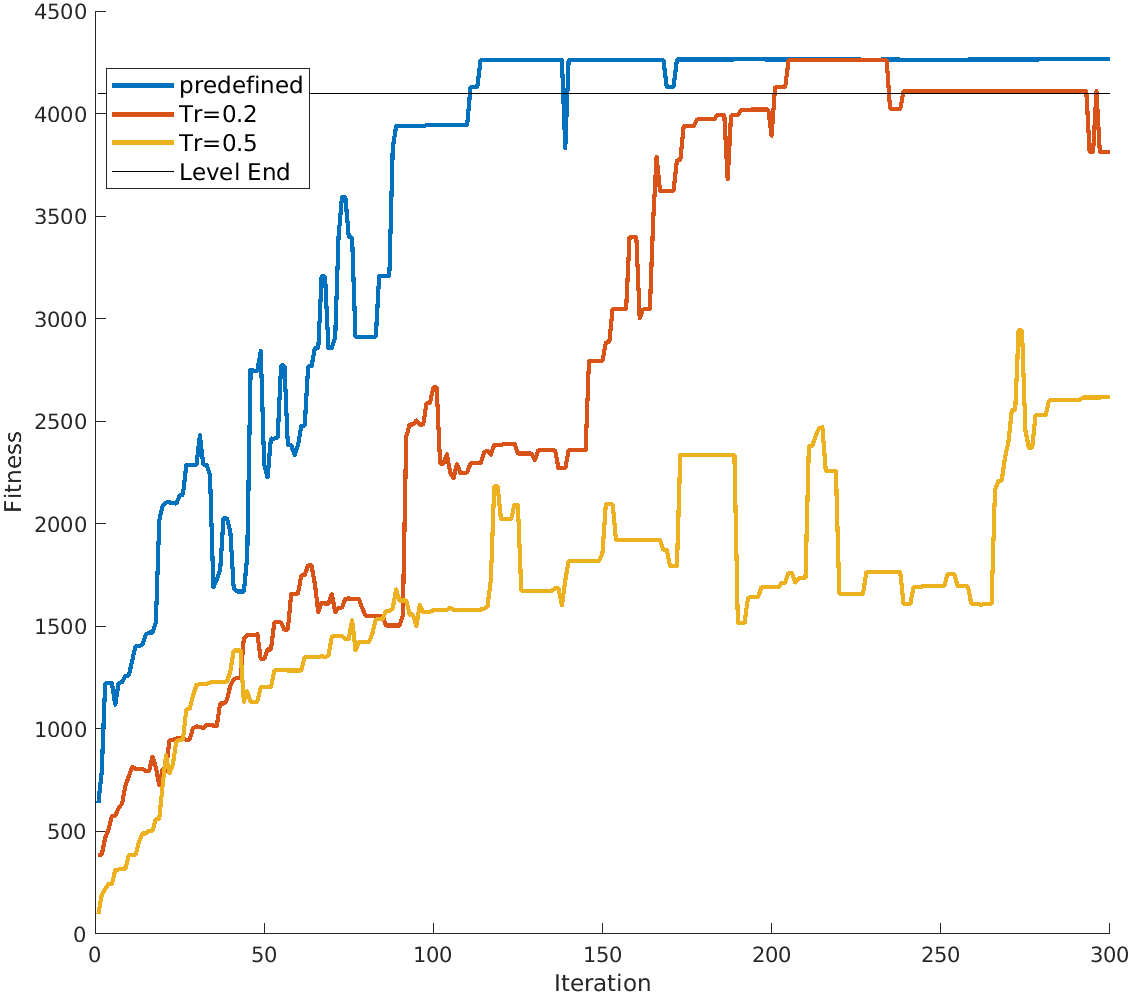
\includegraphics[width=\linewidth]{img/controls.png}
	\caption{Steuervarianten Predefined vs Threshold}
	\label{fig:control}
\end{figure}

\newpage

Des Weiteren haben wir uns angeschaut,  welcher Threshold für den Output genommen werden soll, damit eine Taste gedrückt wird oder nicht. Vermutet hatten wir, dass der Threshold 0,5 am besten sein sollte, da dort der Anstieg der Aktivierungsunktion am größten ist. In Figure \ref{fig:treshold} lässt sich aber erkennen, dass der Durchschnitt über die Elite bei 10 Versuchen bei unterschiedlichen Lernraten immer schlechter ist, als wenn man den Treshold auf 0,2 setzt und dort die unterschiedlichen Lernraten testet. 
\begin{figure}[h!]
	\centering
	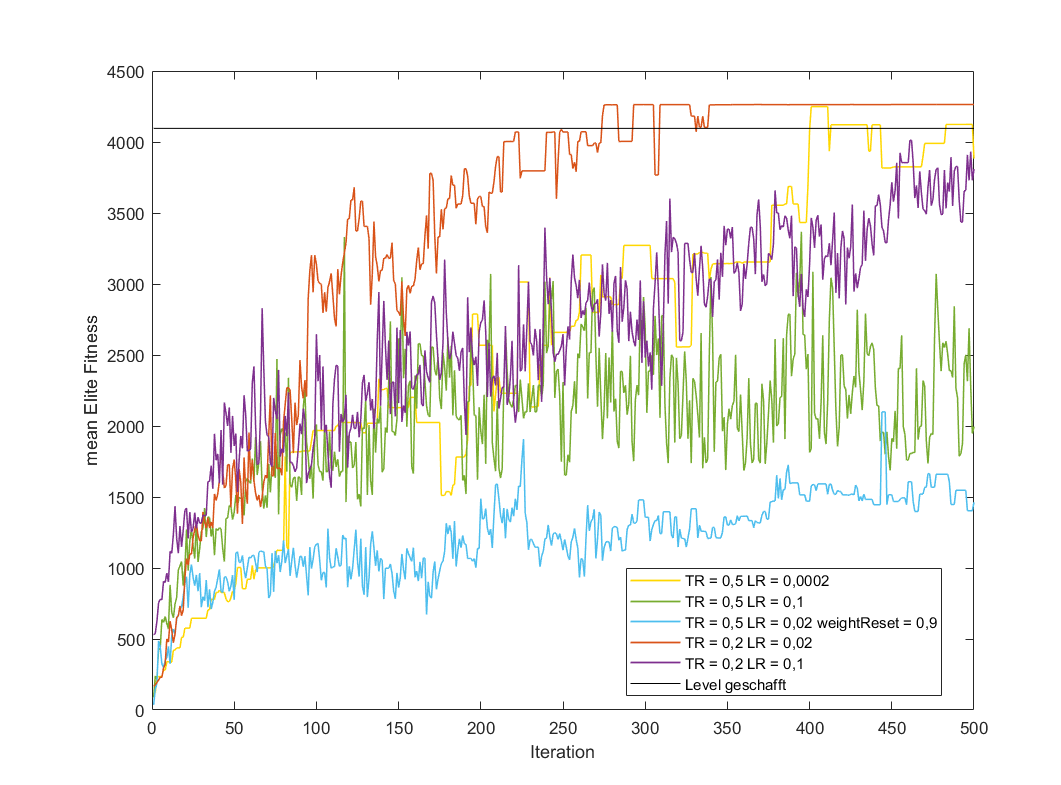
\includegraphics[width=\linewidth]{img/Mario_Treshold.png}
	\caption{Durchschnitt der Elite bei 5 Wiederholungen beim Vergleich von unterschiedlichen Tresholds im Zusammenspiel mit unterschiedlichen Lernraten}
	\label{fig:treshold} 
\end{figure}

Der Boxplot zu dem Experiment zeigt, dass nicht nur die Elite schlechter ist mit einem Treshold von 0.5, sonder dass die Elite nach 500 Iterationen (siehe Figure \ref{fig:treshold_boxplot}) deutlich stärker verteilt ist. Hieraus lässt sich auch ablesen, dass in allen Setups zwar eine Lösung für das Level gefunden werden kann, aber das nicht zwingend der Fall sein muss. So kann es bei einem Treshold von 0.5 und einer Lernrate von 0.0002 auch passieren, dass die Elite nicht mal 35\% des Levels schafft. Der rechte Boxplot in Figure \ref{fig:treshold_boxplot} zeigt, dass nach 500 Iterationen immer eine Lösung für das Level vorhanden ist, weshalb diese Parameter gewählt werden sollte. Allein aus Figure \ref{fig:treshold} hätte man das nicht direkt entscheiden können, ob die blaue oder die gelbe Kurve die besseren Parameter sind, aber aus dem Boxplot ist dies doch klar ersichtlich.\\

\begin{figure}[h!]
	\centering
	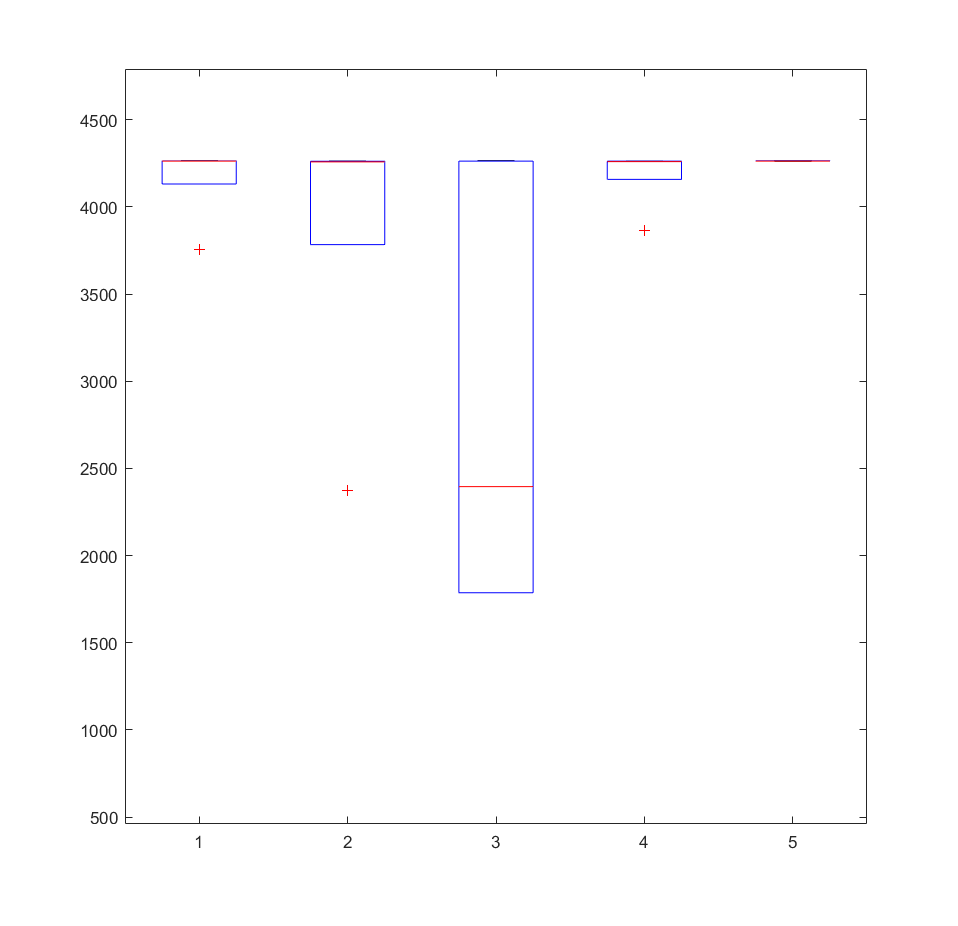
\includegraphics[width=\linewidth]{img/Mario_Treshold_boxplot.png}
	\caption{Boxplot der Elite nach 500 Iterationen von den unterschiedlichen Setups}
	\label{fig:treshold_boxplot} 
\end{figure}


\subsection{Experiment Verhältniss Spezienziel \& Populationsgröße}
In einem Experiment haben wir uns angeschaut, wie sich die Elite bei verschieden starker Spezienbildung entwickelt. Dazu haben wir eine feste Populationsgröße gewählt und Messungen mit unterschiedlichen Spezientargets durchgeführt. In Figure \ref{fig:Spezien} ist genau dies zu sehen bei einer Populationsgröße von 80 und Spezientargets von 2/ 8 und 15. D.h. durchschnittlich waren 40/ 10 oder 5 Topologien in einer Spezie. Dabei kann man sehen, dass wenn zu viele Topologien in einer Spezie sind, sich die Elite nicht gut entwickelt (siehe grüne Kurve in Figure \ref{fig:Spezien}), da sich Spezien kreuzen die sehr unterschiedlich sind. \\
\begin{figure}[h!]
\centering
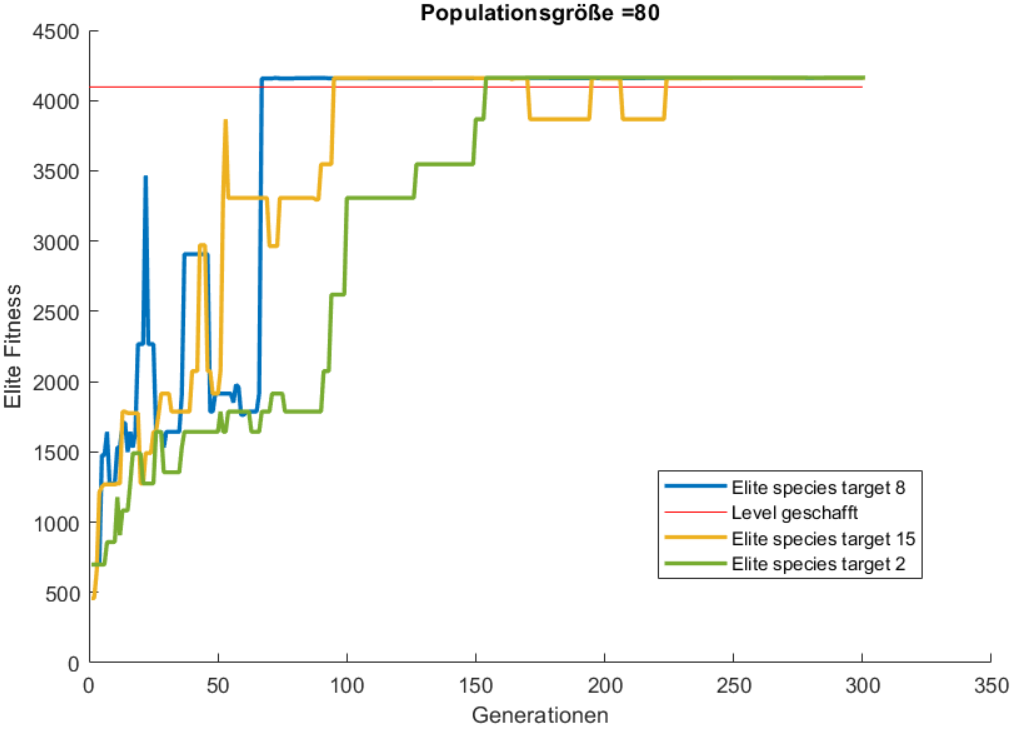
\includegraphics[width=\linewidth]{img/Mario_80_Netze_gesamt.png}
\caption{Experiment mit fester Populationsgröße aber unterschiedlichen Spezientargets}
\label{fig:Spezien} 
\end{figure}

Wenn allerdings zu wenig Topologien in einer Spezie sind ist das für die Entwicklung der Elite auch nicht förderlich. In Figure \ref{fig:Verhaeltniss0_5} sind durchschnittlich 2 Topologien in einer Spezies. Dort kann man feststellen, dass einmal kaum neue Lösungen erzeugt werden(erkennbar durch eine relativ gleichbleibende horizontale Linie am Anfang). Wenn durch Zufall eine neue viel bessere Lösung gefunden wird, passiert es relativ oft, dass diese wieder verworfen wird. Das kommt dadurch, dass die Spezien relativ oft aussterben und sich nicht durchsetzten, da im Schnitt nur 2 in einer sind. Dazu kommt, dass das Kopieren der Elite einer Spezie erst ab einer Größe von 5 passiert, wodurch so auch nicht der beste behalten wird.\\
 
\begin{figure}[h!]
\centering
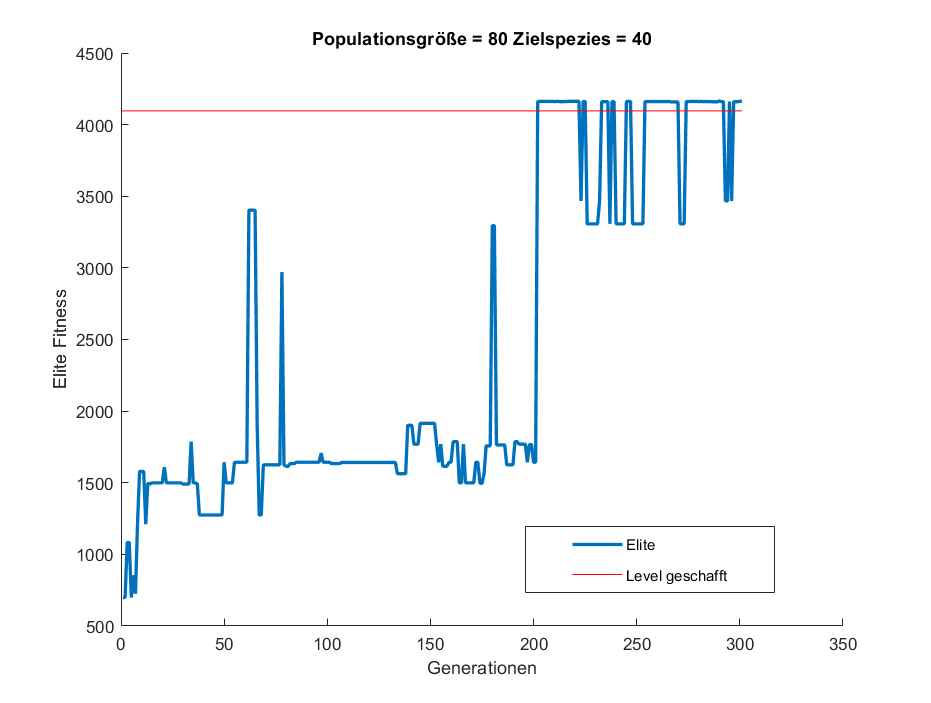
\includegraphics[width=\linewidth]{img/Mario_80_Netze_target_40.png}
\caption{Verlauf der Elite bei einem Verhältnis von 0.5, sodass im Durchschnitt 2 Spezien existieren}
\label{fig:Verhaeltniss0_5} 
\end{figure}



\FloatBarrier
\newpage
\section{Conclusion}


\bibliographystyle{abbrv}
\bibliography{HeteroNEAT} 
\end{document}
}